\documentclass[a4paper,10pt]{article}

\usepackage[margin=3cm]{geometry}
\usepackage[pdftex]{graphicx}

\begin{document}

\title{
  {\normalsize
    Introduction to Algorithms, Data Structures, and Problem Solving\\
    DA4002 (HT11) Halmstad University}\\
  Template Report with Guidelines\\
}
\author{
  \texttt{roland.philippsen@hh.se}
}
\maketitle



\section{Introduction}

a (short!) written report is an essential part of the project.
It must follow a specific format and clearly present the work performed by the team.
In terms of project evaluation, the most important aspects of the report are:
\begin{itemize}
\item Present what has been done by the team during the project.
\item Explain how to run the code developed by the team.
\item Clearly present the obtained technical results.
\end{itemize}
Section~\ref{sec:report} gives detailed guidelines on writing the project report.
The ITADS course focuses on technical aspects of programming and problem solving.
The quality of the written language in the report is secondary, and as long as it remains comprehensible, English errors are not relevant.
Verbatim quotes (copy-pasting) from other sources is acceptable \textbf{if they are short, properly marked, and adequately cited}.
If language is a major obstacle for a team, it is possible to receive a deadline extension for the report only.
Notify the lecturer as early as possible in order to arrange such an extension.

\begin{itemize}
\item course information: University name; course name, code, and date.
\item team information: names, email addresses, study programme
\item project title and subtitle
\item introduction
\item implementation
\item results
\item discussion
\item references
\item quotes
\end{itemize}




\section*{RECYCLE}




\begin{figure}
  \centering
  \fbox{
    \begin{minipage}{0.8\columnwidth}
      \footnotesize
      \verbatiminput{console-ExampleA.txt}
  \end{minipage}}
  \caption{
    Typical console output from \texttt{ExampleA}.
    The table with the running times gives feedback while the benchmark is being run.
    The list of commands at the end allows to view and create figures.
  }\label{fig:exa-console}
\end{figure}
  
\begin{figure}
  \centering
  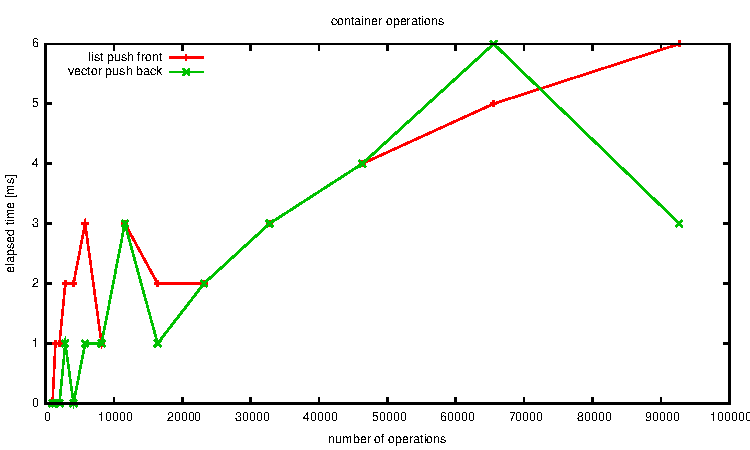
\includegraphics[width=0.8\columnwidth]{plot-ExampleA.pdf}
  \caption{
    Execution time plot produced by running example A.
  }\label{fig:exa-plot}
\end{figure}

It produces console output similar to the one shown in figure~\ref{fig:exa-console}.

Figure~\ref{fig:exa-plot} was produced by running the automatically generated ``\texttt{gnuplot log-1316350931155-all-pdf.plot}'' command.


\begin{figure}
  \centering
  \fbox{
    \begin{minipage}{0.8\columnwidth}
      \footnotesize
      \verbatiminput{console-ExampleB.txt}
  \end{minipage}}
  \caption{
    Typical console output from \texttt{ExampleB}.
    Similarly to figure~\ref{fig:exa-console}, the table is produced while the benchmark is being run.
    Again, the list of commands at the end allows to view and create figures.
  }\label{fig:exb-console}
\end{figure}

\begin{figure}
  \centering
  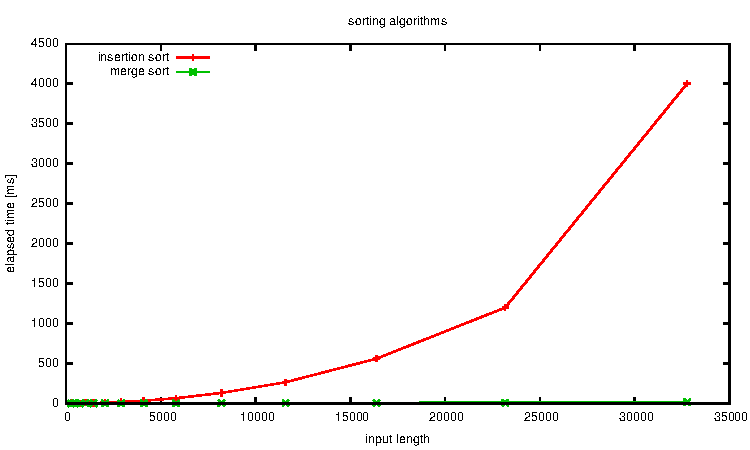
\includegraphics[width=0.8\columnwidth]{plot-ExampleB-all.pdf}\\
  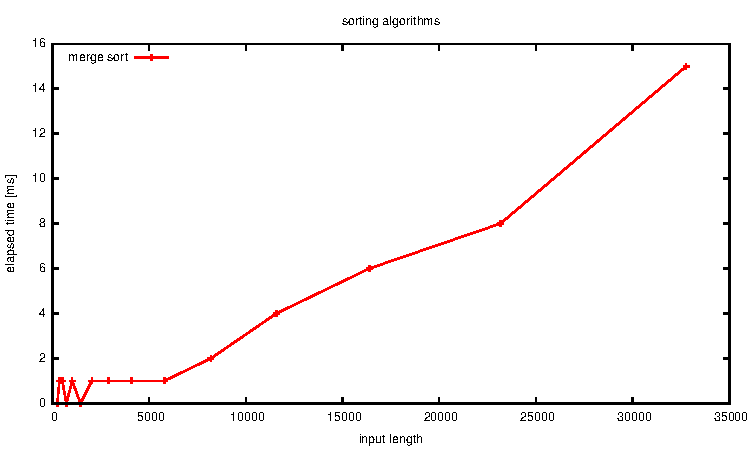
\includegraphics[width=0.8\columnwidth]{plot-ExampleB-zoom.pdf}
  \caption{
    Execution time plot produced by running example B.
    The bottom figure is a zoom on the running time of merge sort.
  }\label{fig:exb-plot}
\end{figure}

It produces console output like the one in figure~\ref{fig:exb-console}.

Figure~\ref{fig:exb-plot} shows two figures based on this run, produced with the two PDF plot scripts mentioned in the console output.

\cite{wikipedia:merge-sort,wikipedia:insertion-sort,wikipedia:bubble-sort}



\footnotesize
\bibliographystyle{plain}
\bibliography{itads-bibliography}


\end{document}
